%!TEX root = ../template.tex
%%%%%%%%%%%%%%%%%%%%%%%%%%%%%%%%%%%%%%%%%%%%%%%%%%%%%%%%%%%%%%%%%%%%
%% chapter.tex
%% NOVA thesis document file
%%
%% Chapter with solution proposal
%%%%%%%%%%%%%%%%%%%%%%%%%%%%%%%%%%%%%%%%%%%%%%%%%%%%%%%%%%%%%%%%%%%%
\chapter{USE-ME evaluation}
\label{cha:evaluation}

% \section{USE-ME evaluation}	
% \label{sec:evaluation}
% (source: CAT Section 4.2.1)

    We used experts feedback as a form of evaluating \gls{useme}, concerning its usefulness. This evaluation was itself planned using \gls{useme}, to express the context and usability objectives of the \gls{useme} support (introduced in chapter \ref{cha:prototype}), as well as to model the expert evaluation and present results.
    %It was necessary to systematically obtain a experts feedback about the feasibility and usefulness of the methodology proposed in the context of this thesis. We use our approach to express the context and usability objectives of the \gls{useme} support (introduced in Chapter \ref{cha:prototype}), as well as to model the expert evaluation and present results. 
    The model instantiation 
    (\textit{pt.fct.unl.novalincs.useme.example.UseMe}) can be found in \gls{useme} GitHub repository: github.com/akki55/useme/tree/master/examples/.
    
    \section{USE-ME context and goal model}
    \label{sec:UsemeContextGoal}
    In this Section, we specify the context of use which we considered while building a \gls{useme} tool support and which justifies our design decisions. 
    
        \subsection{User hierarchy and user profiles}
        \label{sec:usemeProfile}
    
            First, we defined the user profiles which are considered to use the \gls{useme} conceptual framework. 
            
            Figure \ref{fig:UseMeHierarchy} presents the user hierarchy, for which we define several User profiles.
            We characterized any \gls{useme} Stakeholder with a Profile template reflecting demographics, which contains the following classifiers:
            \begin{itemize}
                \item Age - a factor which can indicate if there are users of certain age groups which can adapt systematic approach easier. However, the conceptual framework is not considering the stakeholders which are children (under 18 years).
                \item Country - factor which can influence the user adoption of the conceptual framework with properties of certain country (e.g. education system, accessibility of information, necessity of adoption of the \gls{useme} conceptual framework)
                \item Institution - factor which can influence the user adoption of the conceptual framework with properties of the certain institution 
                \item Degree - the level of education moderates the ability to deal with the complexity of the conceptual framework %level of education is important factor when comprehending the complexity of conceptual framework
                \item Experience background - 
                allows assessing the extent to which people coming from different contexts (e.g. academic (i.e. research) or industrial (i.e. practical)) influences their perception and objectives while assessing \gls{useme}.
                \item E-Mail - person's identifier/contact
                \item Name - person's secondary identifier
                \item Personal Page - person's personal web page
                \item Role - role which person is taking in relation to \gls{useme} development
            \end{itemize}
           
            \begin{figure}[h]
            \centering
            %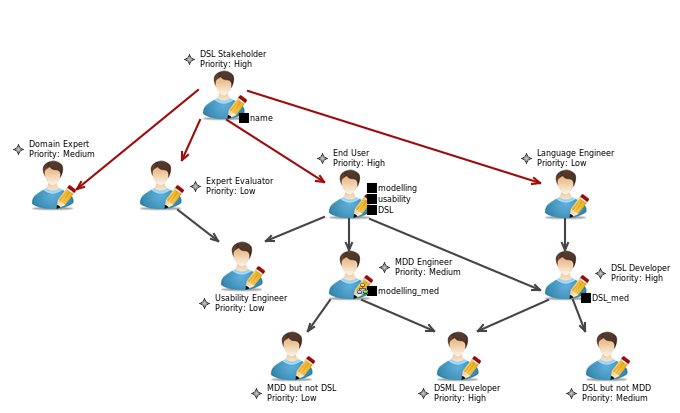
\includegraphics[width=0.5\textwidth, trim=0.6cm 0.6cm 0.0cm 0.6cm, clip]{Figures/USE-ME UserHierarchy.pdf}
            \includegraphics[width=1\textwidth]{Chapters/Figures/USE-MEUserHierarchy.pdf}
            \caption{USE-ME User Hierarchy diagram}
            \label{fig:UseMeHierarchy}
            \end{figure}
            
            The thesis candidate played a double role in \gls{useme} development, as a \textbf{Language Engineer} and \textbf{Expert Evaluator}, while the supervisors of the thesis played the role of \textbf{Domain Experts}. 
            The \textbf{End User} profile represents people not involved in \gls{useme} development, but who are potential users of \gls{useme}, as software language engineers.
            %represent the persons which were not included in \gls{useme} development. 
            It is classified into a three sub-profiles, in regard to their knowledge about modelling, usability or \gls{dsl}s and characterized by a profile template which reflects the relevant knowledge about:
            \begin{itemize}
                \item \gls{dsl} - as the \gls{useme} conceptual framework is intended for \gls{dsl} development
                \item Modelling - as the \gls{useme} conceptual framework is developed using \gls{mdd} approach
                \item Usability - as the \gls{useme} conceptual framework is developed to support usability evaluation
                \item \gls{uml} - as the \gls{useme} conceptual framework is specified by \gls{uml} diagrams
                \item Requirement Engineering - as the \gls{useme} conceptual framework is supporting the validation of usability goals and requirements (e.g. categorized as non-functional in requirement engineering), and therefore is based on requirement engineering goal modelling practice
                \item Agile Development - as the \gls{useme} conceptual framework is meant to be applied iteratively and incrementally
                \item \gls{hci} - as the usability evaluations are meant to improve \gls{hci} between a user (i.e End User) and a software product (i.e. \gls{dsl}).
            \end{itemize}
            
            
            The \textbf{\gls{dsl} Developer} profile is expected to have a medium to high knowledge regarding \gls{dsl} development and has the highest priority to be evaluated, as it represents a primary group of users which are considered to benefit with the adoption of \gls{useme} conceptual framework.
              
            The \textbf{\gls{mdd} Engineer} profile is expected to have a medium to high knowledge regarding modelling techniques and has a medium priority to be evaluated, as it represents a group of users related to \gls{mdd}, and \gls{useme} support was built using this approach.
            
            
            The \textbf{Usability Engineer} profile is expected to have a medium to high knowledge regarding usability and has a low priority to be evaluated. This is because the Usability Engineers are not often included in \gls{dsl} development, so they do not represent a primary group of users. When there is a possibility to introduce them into the development process of a \gls{dsl} they will play a role that fits well with the tasks supported by \gls{useme}. 
            It should be noted that Usability Engineers will often not be  experienced, or even trained in modelling, or \gls{dsl} development.
            %However, they might lack a knowledge about modelling or \gls{dsl} development.
            
            The \textbf{DSML Developer} profile is a child profile of \gls{dsl} Developer and \gls{mdd} Engineer. It has a high priority as it is a primary user of a \gls{useme} conceptual framework, having at least medium knowledge about \gls{dsl} development and MDD.
    
        \subsection{Context environment}
            
            While developing the \gls{useme} framework we took into  account the following environmental considerations (which are represented in Figure \ref{fig:UseMeEnvironmentContext}):
            \begin{itemize}
                \item Technical Environment - The \gls{useme} support is built using \gls{mdd} approach and is designed to be run over a Modeling environment which requires an Operatitng System (OS). The support was built using \gls{emf} and the visual representation of models is supported by Sirius. The \gls{useme} is meant to be used over any OS supporting \gls{emf} and Sirius (e.g. Windows, Mac or Linux).
                \item Social Environment - The \gls{useme} is developed and presented in the English language.
                \item Physical Environment - To use \gls{useme} a Computer should be used, having a RAM and Processor power which is required by the Modeling environment. From Interaction devices, it is mandatory to use the mouse and keyboard. 
            \end{itemize}
    
            
            \begin{figure}[h]
            \centering
            \includegraphics[width=1\textwidth]{Chapters/Figures/USE-MEEnvironmentContext.pdf}
            \caption{USE-ME Context Environment diagram}
            \label{fig:UseMeEnvironmentContext}
            \end{figure}
            
            \subsection{Workflows}
            
            During the development of \gls{useme} prototype we found the following three workflows to be mandatory:
            \begin{itemize}
                \item [W1] \texttt{\gls{dsl} Usability Evaluation} -  represent the main objective of the \gls{useme} framework for any end user and is prioritized as High, indicating that should be evaluated in the development cycle addressed in the context of this thesis.
                \item [W2] \texttt{Integration with \gls{dsl} development artifacts} - the idea of the \gls{useme} conceptual framework is to be integrated with the \gls{dsl} development cycle (see Figure \ref{fig:UseMeWorkflows}). It is beneficial for any \gls{dsl} developer to integrate existing development artefacts and enable an information exchange to assure the real-time updates and traceability of the impact of usability evaluation to complete \gls{dsl} development scope.
                \item[W3] \texttt{Integration with experimental analysis tools} - The \gls{useme} conceptual framework is designed in a way to connect its testing instruments with third party applications for survey design, events capturing, or data analysis, among others.
                %with existing applications for a survey design, events capturing or a statistical analysis of the tools.  
                It is expected to support an integration between specifications provided by \gls{useme} and and by existing experimental support (e.g. importing/exporting the questionnaire forms automatically between \gls{useme} and Google Forms).  
            \end{itemize}
            
             \begin{figure}[h]
            \centering
            \includegraphics[width=1\textwidth]{Chapters/Figures/USE-MEWorkflows.pdf}
            \caption{USE-ME Workflows diagram}
            \label{fig:UseMeWorkflows}
            \end{figure}
            
            We break the workflow W1 (see Figure \ref{fig:UseMeScenario}) into the several independent scenarios specified for \gls{useme} conceptual framework in a form of activity diagrams (see Chapter \ref{cha:useme}), namely Context Modelling, Goal Modelling, Evaluation Modelling which includes Survey Modelling or/and Interaction Modelling, and Result Modelling. 
    
             \begin{figure}[h]
            \centering
            \includegraphics[width=1\textwidth]{Chapters/Figures/USE-MEWorkflowScenarios.pdf}
            \caption{USE-ME Scenario diagram}
            \label{fig:UseMeScenario}
            \end{figure}
        
        
        \subsection{Goal model}
        \label{sec:usemeGoal}
        
            The main objective of developing the \gls{useme} conceptual framework was to address three research questions which were introduced in a Section \ref{sec:problems}. We proposed \gls{useme} methodological conceptual framework and associated prototype tool as solutions to our research problems. 
            Achieving a high level of quality in use of the \gls{useme} conceptual framework is very important in order to be adopted by the intended community (i.e. \gls{useme} potential End User presented in Figure \ref{fig:UseMeHierarchy}). In order to achieve a high level of usability, the conceptual framework should be presented in a comprehensive way, as well as supported with a tool which is understandable from the perspective of End Users, especially \gls{dsl} developers. 
        
        \begin{figure}[h]
            \centering
            \includegraphics[width=1\textwidth]{Chapters/Figures/USE-MEUsabilityGoalModel.pdf}
            \caption{USE-ME goal model}
            \label{fig:UseMeGoal}
            \end{figure}
        
            In the context of the work presented in this thesis, we  evaluate the usability goal associated with the workflow \textbf{W1} '\gls{dsl} Usability Evaluation' (Figure \ref{fig:UseMeScenario}).  All stakeholders included in \gls{useme} development are responsible for achievement of this goal (see Figure \ref{fig:UseMeGoal}), however, we define its subgoal for which just Evaluation Expert is responsible for 'Usability of the performing \gls{dsl} Usability evaluation'. The first step in achieving this goal was to capture all the relevant concepts and provide comprehensive specifications. This way we ensure to build the language which is \textit{expressive} enough to support various activities which are necessary to be performed for different types of usability assessments. Further, we built supporting tool which is {feasible} to instantiate a usability evaluation assessment into model (Chapter \ref{cha:prototype}).
        
            The second goal is defined to address the 'Integrability with \gls{dsl} artefacts', and is important to be addressed in later phases of development. By achieving this goal we expect to facilitate the process of reusing already obtained information about \gls{dsl} development, which is stored within its artefacts. For instance, information which shapes the context definition can already be found in \gls{dsl} artefacts like the feature diagrams, use-case/scenario descriptions, process documentation, etc. The usability goal model by itself ideally should be integrated with an existing goal model of the \gls{dsl}, in which it is enabling the specification and assessment of context-aware goals. 
        
            Finally, the third goal is defined to address the 'Integrability with tools which support experimental analysis', which should enable the <End User> to automatically generate evaluation instruments, and import the results in the result models. This integration possibility will enable faster and safer implementation of the test models and save the time in importing the obtained data. 
    
        \section{USE-ME evaluation model}
           % \lablel{sec:UseMeEvaluation}
            
            %Evaluation of the presented methodology was performed in several steps which are described in the Section \ref{sec:methodology}. 
            
            %We conducted a multiple-case study in order validate the proposed method; two academic case studies served to specify and confirm the evaluation model and experiment designs\cite{Barisic2012plateu, barisic2016stsm}; two industrial case studies were used to apply the approach during iterative real case development \cite{barisic2014flows, BarisicVisualinoURL}. The researcher was not included in DSL development but was taking a role of expert evaluator. 
            
            %Early evaluations showed to be beneficial and integrable with an agile development process of FlowSL \cite{barisic2014flows}. The controlled experiments on several releases of a Visualino \cite{BarisicVisualinoURL} showed reuse of the evaluation model instances and significant improvements in usability.
        
            %Finally, we combined approach with an existing requirement engineering approach for DSLs to show it's \textit{integrability} with existing DSL development support \cite{barisic2017RDAL}
            
            
            To evaluate the \textit{feasibility} of adopting \gls{useme} conceptual framework, we developed tool support integrable into \gls{dsl} development infrastructure \cite{barisic2017UseMe1.1} and illustrated an instantiation
            of prototype models on the Visualino case study \cite{barisic2017UseMeJournal}.
            The prototype was validated in the context of projects for a \gls{dsl}s graduate course \cite{barisic2017pilot}, helping novice language engineers (i.e. master students) to prepare \gls{dsl} evaluations (see Chapter \ref{cha:prototype}).
            
            To evaluate how well the \gls{useme} conceptual framework and associated prototype addressed our research problems, presented in Section \ref{sec:problems}, we gathered opinions from more experienced potential \gls{useme} users. We performed our evaluation with two complementary instruments:
            \begin{itemize}
                \item \emph{Evaluation interview.} A detailed interview will be run with people who used our systematic approach in its current, or an earlier phase. We have contacted the candidates by their personal contact and shared with them the conceptual framework proposal (Annex \ref{ann:Visualino}). The objective of the interview was to obtain feedback about participants experience while applying usability evaluation methods in the context of the \gls{dsl} they were developing, as well as, to obtain a general feedback about the \gls{useme} framework. 
                \item \emph{Evaluation survey.} The evaluation questionnaire will be run with people which are experienced in \gls{mdd} and \gls{dsl} development or/and with \gls{hci} and empirical studies. 
        
            \end{itemize}
            
            
            
               \subsection{Evaluation subjects and context}
               
               The evaluation targets  people experienced in research, who obtained the master or doctoral degree. The participants are expected to fit some of the [End User] profiles, which have a relevant knowledge in usability, modelling or \gls{dsl} development (see Section \ref{sec:usemeProfile}). 
        
                As we targeted more senior people in research, who are usually not available to spend a lot of time, we decided to run the evaluation survey [Online] and keep it short as possible. It was not necessary to set up a technical environment, although the tool was used in a presentation. However, participants were expected to speak English and needed to use a computer and a web browser and web access.% As it was the online evaluation survey, participants were required to have an access to network.   
                
                We invited  people with the following profiles to participate:
                \begin{itemize}
                    \item people familiar with our systematic approach in its current or an earlier phase (e.g. ones that were making part of \gls{dsl} development for the case studies where we applied \gls{useme} conceptual framework, or were applying it independently in its early phase);
                    \item people from the networks related to \gls{dsl} development {like DSM-TP\footnote{msdl.cs.mcgill.ca/conferences/dsm-tp-2017 (accessed September 19, 2017)} summer school, MPM4CPS\footnote{http://mpm4cps.eu/ (accessed September 19, 2017)} COST IC1404 action members or the DSM Forum\footnote{http://www.dsmforum.org/ (accessed September 19, 2017)}};
                    \item people we cited in our references for which we had e-mail, or a profile in social networks like LinkedIn \footnote{www.linkedin.com (accessed September 19, 2017)} and Research Gate\footnote{www.researchgate.net (accessed September 19, 2017)};
                    \item people recommended by the other participants.
                \end{itemize}
                In total we invited over 350 persons using their personal contact reference. 
                Also, we made the link accessible at \gls{useme} GitHub wiki page \footnote{github.com/akki55/useme/wiki (accessed September 19, 2017)} and all participants were invited to share the link further. We reproduce here the letter of invitation which was shared with potential participants. 
                
                \textbf{'Invitation to provide a feedback about usability evaluation modelling framework for Domain-Specific Languages'}
        
                \emph{'SURVEY LINK: https://goo.gl/forms/Js4Nh8V6VCZvmsAB2}
                
                \emph{This experimental work is conducted within the NOVA Laboratory for Computer Science and Informatics (NOVA LINCS) in the context of the evaluation of \gls{useme} conceptual framework which was developed as a part of the PhD thesis. }
        
                \emph{We hope that you may find it interesting to contribute by providing your opinion about the provided solution. We are searching mainly for people which have background knowledge about domain-specific languages, model-driven development, human-computer interaction, empirical studies OR usability testing. However, anyone interested in the topic is welcome to participate. I would be also grateful if you could share the invitation link also with colleagues, for which you believe that may find this work interesting.} 
        
                \emph{The experiment will be kept strictly confidential and will be made available only to members of the research team of the study or, in case external quality assessment takes place, to assessors under the same confidentiality conditions. Data collected in this experiment may be part of the final research report, but under no circumstances will your name or any identifying characteristic be included in the report.
                In particular, there is no intention of judging you as a person or the skills and experience that you will use in this survey - the goal is the evaluation of the proposed approach!'}
        
             
            \subsection{Evaluation objectives}
            \label{sec:exObjective}
            
                The objective of this study was to evaluate the goal U1 'Capability to perform \gls{dsl} usability evaluation' in regard to If it is \textit{feasible} for <\gls{dsl} Developers> to perform \gls{dsl} usability evaluation with \gls{useme}. We associate with this goal our three research questions defined in (Section \ref{sec:rq}) and define the following evaluation goals and their associated question as follows:
                
                \begin{itemize}
                    \item [\textbf{G1}] Does the \gls{useme} conceptual framework enable End Users to model \gls{dsl} usability evaluations?
                
                    \item [\textbf{G2}] Does the \gls{useme} conceptual framework enable End Users in promoting usability concerns since an early stage of \gls{dsl} development
                
                    \item [\textbf{G3}] Does the \gls{useme} tool support enable End Users to built usability evaluation into the development process of the \gls{dsl}
                \end{itemize}
                
                The evaluation goal [\textbf{G1}] is associated with RQ1, and we specify the problem which it aims to solve in form of Goal-Quality-Metric (GQM) \cite{van2002goal} format:
                \textit{'Analyze the effect of the [\gls{useme} conceptual framework], for the purpose of evaluation, with respect to its impact on the [feasibility]  to model the \gls{dsl} usability evaluation, from the point of view of the [researcher], in the context of the evaluation survey conducted with [End User].}
                %We specify the alternative and null hypotheses for evaluation goal [\textbf{G1}] as:
                
                %\begin{itemize}
                 %   \item  \textit{H1\_null}: Using [\gls{useme} conceptual framework] has no influence on the [feasibility] of [End Users] modelling \gls{dsl} usability evaluations.
              
                  %  \item \textit{H1\_{alt}}: Using [\gls{useme} conceptual framework] impacts the [feasibility] of [End Users] modelling \gls{dsl} usability evaluations.
                %\end{itemize}
                
                The evaluation goal [\textbf{G2}] is associated with RQ2, and associated problem statement is defined as:
                \textit{'Analyze the effect of the [\gls{useme} conceptual framework], for the purpose of evaluation, with respect to its impact on [feasibility]  to promote usability concerns since an early stage of \gls{dsl} development, from the point of view of the [researcher], in the context of the {online} evaluation survey conducted with [End User].}
                %We specify the alternative and null hypotheses for evaluation goal [\textbf{G2}] as:
                
                %\begin{itemize}
                 %   \item  \textit{H2\_null}: Using [\gls{useme} conceptual framework] has no influence on the [feasibility] of [End Users] to promote usability concerns since an early stage of \gls{dsl} development.
              
                  %  \item \textit{H2\_{alt}}: Using [\gls{useme} conceptual framework] impacts the [feasibility] of [End Users] to promote usability concerns since an early stage of \gls{dsl} development.
                %\end{itemize}
                
                The evaluation goal [\textbf{G3}] is associated with RQ3, and we specify problem which it aims to solve in form of Goal-Quality-Metric (GQM) as:
                \textit{'Analyze the effect of the [\gls{useme} tool support], for the purpose of evaluation, with respect to its impact on [feasibility]  to built usability evaluation into the development process of the \gls{dsl}, from the point of view of the [researcher], in the context of the {online} evaluation survey conducted with [End User].}
                %We specify the alternative and null hypotheses for evaluation goal [\textbf{G1}] as:
                
                %\begin{itemize}
                 %   \item  \textit{H3\_null}: Using [\gls{useme} conceptual framework] has no influence on the [feasibility] of [End Users] to built usability evaluation into the development process of the \gls{dsl}.
              
                  %  \item \textit{H3\_{alt}}: Using [\gls{useme} conceptual framework] impacts the [feasibility] of [End Users] to to built usability evaluation into the development process of the \gls{dsl}.
                %\end{itemize}
        
            \subsection{Evaluation process and documentation}
            
                In Figure \ref{fig:SurveyProcess} we introduce the process and documents which were used during the survey execution. All participants needed to watch the presentation video\footnote{youtu.be/RjIGFex-zQM (accessed September 19, 2017)} about the \gls{useme} conceptual framework. We prepared a 15 minutes video in which we introduced the motivation for developing the \gls{useme} conceptual framework, its usage which was illustrated by a specification model from Chapter \ref{cha:useme}, and an instantiation of the evaluation model supported by the \gls{useme} prototype from Chapter \ref{cha:prototype}. All participants were asked to respond the survey questionnaire which we introduce in Section \ref{sec:surveymodel}.
                Finally, they were provided with the \gls{useme} tool \cite{barisic2017UseMe1.1} and the article describing \gls{useme} conceptual framework \cite{barisic2017UseMeJournal} to consult additionally if they would like to invest more time to understand the conceptual framework. 
                
                
                \begin{figure}[h]
                    \centering
                    \includegraphics[width=1\textwidth]{Chapters/Figures/SurveyProcess.png}
                    \caption{Evaluation process}
                    \label{fig:SurveyProcess}
                \end{figure}
                    
                The pilot trial of the survey was executed with our interview candidates and three members of NOVA-LINCS research centre. It was run in the period from July 1, 2017 till July 15, 2017. The participants were asked to access the provided documentation, watch the video tutorial and to answer the survey. All participants from the pilot run rated the materials as complete and easy to understand, and provided small improvement suggestions. Evaluation materials were updated in accordance with provided suggestions after the pilot session was over.
                
                The interview with participants was scheduled in the period from July 15 until July 20, 2017. Interview sessions were conducted individually and participants were asked to allow to be voice recorded. This helped the evaluator to analyse the feedback afterwards and by that shorten the time and increase the quality of the interview. The interpretations which were taken from the interview were given to participants for review to confirm that they were well understood by the evaluator. 
                
                Finally, we run a survey from July 25 till September 12, 2017. after which we analysed and reported the results (see Section \ref{sec:surveyresults}).
         
    
    \section{Survey model}
        \label{sec:surveymodel}
        
        The survey form is reproduced in Annex \ref{ann:surveyForm}. The survey questions are classified in Table \ref{tbl:qsClasf} and categorized as background and feedback questions. Background questions are designed to collect the participant's demographics (DQ) and self-rated experience in the area (EQ). Feedback questions (FQ) are meant to assess the opinion about the motivation and feasibility of the \gls{useme} conceptual framework. Participants were invited first to read an abstract, watch the video tutorial and to check the documentation regarding the \gls{useme} conceptual framework. Like this, they were able to decide upfront if they fit the right profile to provide feedback. After this, participants are asked to fill in the Background questionnaire, followed by the Feedback questionnaire. Finally, they were asked to report on the time which they spent into getting familiar with an conceptual framework, as well the time to fill in the questionnaire. 
        
        % Please add the following required packages to your document preamble:
        % \usepackage[table,xcdraw]{xcolor}
        % If you use beamer only pass "xcolor=table" option, i.e. \documentclass[xcolor=table]{beamer}
        % Question classification
            \begin{table}[]
            \centering
            \caption{Question classification}
            \label{tbl:qsClasf}
            \begin{tabular}{|ll|ll|}
            \hline
            
            \multicolumn{1}{|l|}{\cellcolor[HTML]{C0C0C0}\textbf{Classification:}} & \cellcolor[HTML]{C0C0C0}\textbf{Questions:}   & \multicolumn{1}{l|}{\cellcolor[HTML]{C0C0C0}\textbf{Classification:}} & \cellcolor[HTML]{C0C0C0}\textbf{Questions:}   \\ \hline
            \multicolumn{1}{|l|}{\cellcolor[HTML]{C0C0C0}\textbf{BACKGROUND}}       & \cellcolor[HTML]{C0C0C0}\textbf{DQ,EQ}   & \multicolumn{1}{l|}{\cellcolor[HTML]{C0C0C0}\textbf{FEEDBACK}}      & \cellcolor[HTML]{C0C0C0}\textbf{FQ}  \\ \hline
            \textbf{Demographics}                          & DQ1-DQ9   & \textbf{Motivation}                           & FQ4-FQ8   \\ \hline
            \textbf{Experience}                            & EQ1-EQ23  & \textbf{Feasibility}                          & FQ9-FQ18  \\
            Modelling                                      & EQ4-EQ5   & RQ1                                           & FQ9-FQ12  \\
             \gls{uml}                                            & EQ6-EQ10  & RQ2                                           & FQ13-FQ14 \\
            \gls{dsl}                                            & EQ11-EQ15 & RQ3                                           & FQ15-FQ18 \\ \cline{3-4} 
            Requirement engineering                        & EQ16-EQ17 & \textbf{Suggestions}                          & FQ19                  \\ \cline{3-4} 
            Agile development                              & EQ18                  & \textbf{Usability tools}                      & FQ20                  \\
            \gls{hci}                                            & EQ19-EQ23 &                                               &                       \\ \hline
            \end{tabular}
            \end{table}
            
            In order to quantify answers to our questionnaire, we predefined four different Likert scales in Table \ref{tbl:Scale}. We used DegreeScale, development scale and  experts call as a part of Background Questionnaire. The degree scale was meant to obtain the feedback about the obtained academic degree of our participants. The ExpertScale served for reporting a level of their experience with the relevant approaches or tools. The development scale was used for participants to report their experience with the \gls{dsl} development. We preferred to define this scale in a manner which will reflect the participant's practical experience with the \gls{dsl} development. Finally, we used AgreeScale in the Feedback Questionnaire.
        
    
        % Scale definition    
            \begin{table}[]
            \centering
            \caption{Scales definition}
            \label{tbl:Scale}
            \begin{tabular}{|p{0.15\columnwidth}|p{0.15\columnwidth}|p{0.2\columnwidth}|p{0.4\columnwidth}|}
            \hline
            \cellcolor[HTML]{C0C0C0}\textbf{DegreeScale:} & \cellcolor[HTML]{C0C0C0}\textbf{ExpertScale:}     & \cellcolor[HTML]{C0C0C0}\textbf{AgreeScale:} & \cellcolor[HTML]{C0C0C0}\textbf{DevelopmentScale:}                                               \\ \hline
            PhD                   & Expert                    & Strongly agree       & Yes, I developed few functional \gls{dsl}s of which at least one is widely used \\ \hline
            MSc                   & Advanced                  & Agree                & Yes, I developed a functional \gls{dsl}                                        \\ \hline
            BSc                   & Intermediate              & Don't know           & Yes, I developed few prototypes                                          \\ \hline
            Other                 & Emerging  & Disagree             & Yes, in the context of faculty course                                    \\ \hline
                                  & None                      & Strongly disagree    & No                                                                       \\ \hline
            \end{tabular}
            \end{table}
    
            \subsection{Background questionnaire}
        
            The background questionnaire, defined in the Table \ref{tbl:bckQs}, served for collecting demographics and experience data from the survey participants. The questions are designed to assess the [End User] profile characteristic, which we defined for \gls{useme} context model in Section \ref{sec:usemeProfile}. 
            Information obtained by DQ2, DQ3, DQ4 and DQ9 are kept strictly confidential and served for validation of the persons profile and as a personal contact point. Questions DQ5, DQ6, DQ7 and DQ8 served to highlight the diversity of our participants, as well as their maturity level. 
            
           
        
        
    
            %Background Questionnaire
            \begin{table}[]
            \centering
            \caption{Background Questionnaire}
            \label{tbl:bckQs}
            \begin{tabular}{|l|p{0.7\columnwidth}|l|}
            \hline
            \cellcolor[HTML]{C0C0C0}\textbf{Id}   & \cellcolor[HTML]{C0C0C0}\textbf{Question}                                                                     & \cellcolor[HTML]{C0C0C0}\textbf{Value}      \\ \hline
            \textbf{DQ1}  & Timestamp:                                                                            & Number              \\ \hline
            \textbf{DQ2}  & Email Address:                                                                          & Text                \\ \hline
            \textbf{DQ3}  & Full Name:                                                                          & Text                \\ \hline
            \textbf{DQ4}  & Personal page or public profile:                                                      & Text                \\ \hline
            \textbf{DQ5}  & Age:                                                                                  & Number              \\ \hline
            \textbf{DQ6}  & Country:                                                                              & Text                \\ \hline
            \textbf{DQ7}  & Degree:                                                                               & DegreeScale         \\ \hline
            \textbf{DQ8}  & Current Work/Research Position::                                                                             & Text                \\ \hline
            \textbf{DQ9}  & Current Work/Research Institution:                                                                          & Text                \\ \hline
            \textbf{EQ1}  & Experience background:                                                                & Academic / Industry \\ \hline
            \textbf{EQ2}  & How many years of working experience do you have?                                        & Number              \\ \hline
            \textbf{EQ3}  & How many years of research experience do you have?                                       & Number              \\ \hline
            \textbf{EQ4}  & How would you rate your level of knowledge related to modelling techniques?           & ExpertScale         \\ \hline
            \textbf{EQ5}  & How would you rate your experience related to Model-Driven Development \gls{mdd})?         & ExpertScale         \\ \hline
            \textbf{EQ6}  & How would you rate your level of knowledge regarding  \gls{uml}?                             & ExpertScale         \\ \hline
            \textbf{EQ7}  & How experienced are you with modelling use cases?                                     & ExpertScale         \\ \hline
            \textbf{EQ8}  & How experienced are you with  \gls{uml} activity or process diagrams?                        & ExpertScale         \\ \hline
            \textbf{EQ9}  & How experienced are you with  \gls{uml} class diagrams?                                      & ExpertScale         \\ \hline
            \textbf{EQ10} & Are you familiar with modelling interaction (communication) diagrams?                 & ExpertScale         \\ \hline
            \textbf{EQ11} & How would you rate your level of knowledge related to Domain-Specific Languages(DSL)? & ExpertScale         \\ \hline
            \textbf{EQ12} & Did you ever develop a \gls{dsl}?                                                           & DevelopmentScale    \\ \hline
            \textbf{EQ13} & How would you rate your level of knowledge regarding the Eclipse working environment?     & ExpertScale         \\ \hline
            \textbf{EQ14} & How experienced are you with the Eclipse Modeling Framework (EMF)?                        & ExpertScale         \\ \hline
            \textbf{EQ15} & How experienced are you with the Sirius Modeling tool?                                    & ExpertScale         \\ \hline
            \textbf{EQ16} & How experienced are you with software requirements engineering?                       & ExpertScale         \\ \hline
            \textbf{EQ17} & How familiar are you with goal-oriented requirements approaches?                      & ExpertScale         \\ \hline
            \textbf{EQ18} & How experienced are you with agile development?                                       & ExpertScale         \\ \hline
            \textbf{EQ19} & How would you rate your level of knowledge regarding Human-Computer Interaction?      & ExpertScale         \\ \hline
            \textbf{EQ20} & How experienced are you with User-Centered design techniques?                         & ExpertScale         \\ \hline
            \textbf{EQ21} & How familiar are you with empirical experiments?                                          & ExpertScale         \\ \hline
            \textbf{EQ22} & How familiar are you with usability testing?                                              & ExpertScale         \\ \hline
            \textbf{EQ23} & Can you describe (refer to) your previous \gls{hci} experience?                                  & Text                \\ \hline
            \end{tabular}   
            \end{table}
            
               % \item[\textbf{RQ1:}] How are we able to model the \gls{dsl} usability evaluation?
                %\item[\textbf{RQ2:}] How can we promote usability concerns since an early stage of development of the \gls{dsl}?
                %\item[\textbf{RQ3:}] How can we integrate the proposed methodological approach to build usability evaluation into the development process of the \gls{dsl}?
                
                 Experience questions reflect a self-rated Expertise scale (\emph{ExpertScale}) of the participant regarding his/her knowledge of skills which are relevant for understanding and applying the \gls{useme} conceptual framework. These skills are classified into a knowledge of Modelling,  \gls{uml}, \gls{dsl}, Requirement Engineering, Agile development and \gls{hci}, as we classified in Table \ref{tbl:qsClasf}.
                 The combination of this skills reflects the experience sets which are expected from the language engineer or/and the expert evaluator, participating in any \gls{dsl} development project, according to \gls{useme}. 
                 
                 First, we asked the participants to report on their working and research experience (EQ1, EQ3). 
                 To assess the participant's knowledge about Modelling we ask them to rate their experience of modelling in general, as well as with the  \gls{mdd} (EQ4, EQ5). Further, we asked participants to report on their knowledge regarding the \gls{uml} in general (EQ6) and experience with different \gls{uml} diagrams (EQ7, EQ8, EQ9, EQ10). The next question aimed to assess the experience of participants with \gls{dsl} in general (EQ11), as well as with practical development of \gls{dsl}s (EQ12), in particular, knowledge of Eclipse working environment, \gls{emf} and Sirius (EQ13, EQ14, EQ15), which were the tools which used while developing the \gls{useme} prototype. Further, we assessed the participant's knowledge regarding requirement engineering (EQ16, EQ17) and agile development (EQ18). Finally, we wanted to assess their background regarding \gls{hci} (EQ19), of which in particular the \gls{ucd}, empirical experiments and usability testing (EQ20, EQ21, EQ22).
                
                
                 % Please add the following required packages to your document preamble:
            % \usepackage[normalem]{ulem}
            % \useunder{\uline}{\ul}{}
            % Feedback Questionnaire
            \begin{table}[]
            \centering
            \caption{Feedback Questionnaire}
            \label{tbl:feedQs}
            \begin{tabular}{|l|p{0.7\columnwidth}|l|}
            \hline
            \cellcolor[HTML]{C0C0C0}\textbf{Id}   & \cellcolor[HTML]{C0C0C0}\textbf{Question}                                                                                            & \cellcolor[HTML]{C0C0C0}\textbf{Value} \\ \hline
            \textbf{FQ1}  & Did you watch the presentation video?                                                                        & Yes/No         \\ \hline
            \textbf{FQ2}  & Did you read the paper presenting the conceptual framework?                                                              & Yes/No         \\ \hline
            \textbf{FQ3}  & Did you try to use the tool?                                                                                 & Yes/No         \\ \hline
            \textbf{FQ4}  & There is a lack of systematic approach for evaluation of \gls{dsl}s                                                & AgreeScale     \\ \hline
            \textbf{FQ5}  & Usability evaluations are necessary for a \gls{dsl} development in practice                                        & AgreeScale     \\ \hline
            \textbf{FQ6}  & Current usability evaluations of \gls{dsl}s are too expensive and not reusable.                                  & AgreeScale     \\ \hline
            
            \textbf{FQ7}  & It is necessary to specify explicitly a context of the \gls{dsl} when evaluating its usability                                 & AgreeScale     \\ \hline
            \textbf{FQ8}  & \gls{dsl} evolution cycle should include usability re-evaluation                                                   & AgreeScale     \\ \hline
            \textbf{FQ9}  & The provided approach supports modelling of the usability evaluation process for \gls{dsl}s                                  & AgreeScale     \\ \hline
            \textbf{FQ10}  & Concepts modelled by the \gls{useme} framework are relevant for \gls{dsl} development                                       & AgreeScale     \\ \hline
            \textbf{FQ11} & The \gls{useme} approach is easy to understand                                                                    & AgreeScale     \\ \hline
           % \textbf{FQ12} & Can you please explain what did you find difficult, or hard to understand about the \gls{useme} approach:         & Text           \\ \hline
            \textbf{FQ12} & The approach is independent of the particular \gls{dsl} development approach                                       & AgreeScale     \\ \hline
            \textbf{FQ13} & Approach is suitable to be applied from the early stage of the development of the \gls{dsl}                        & AgreeScale     \\ \hline
            \textbf{FQ14} & \gls{dsl}s targeting large user groups can benefit from the investment in application of the \gls{useme} approach iteratively & AgreeScale     \\ \hline
            \textbf{FQ15} & The \gls{useme} tool makes it feasible for a \gls{dsl}  engineer to model a usability evaluation                       & AgreeScale     \\ \hline
            \textbf{FQ16} & The \gls{useme} tool is expressive enough for specifying usability evaluation of \gls{dsl}                              & AgreeScale     \\ \hline
            \textbf{FQ17} & The \gls{useme} tool supports the integration of usability evaluation approach into development process of the \gls{dsl} & AgreeScale     \\ \hline
            \textbf{FQ18} & Investment into the development of the \gls{useme} prototype tool into real product is worthy                      & AgreeScale     \\ \hline
            \textbf{FQ19} & Can you please provide your suggestions concerning how to improve the \gls{useme} tool or approach itself:                   & Text           \\ \hline
            \textbf{FQ20} & Are you familiar with any other tool which supports usability evaluation?                                    & Yes/No         \\ \hline
            FQ20\_1       & What are the other tools you are familiar with?                                                              & Text           \\ \hline
            FQ20\_2       & The \gls{useme} is more suitable then alternatives for usability evaluation of \gls{dsl}s     & AgreeScale     \\ \hline
            FQ20\_3       & The \gls{useme} is more complete then alternatives for usability evaluation of \gls{dsl}s                                   & AgreeScale     \\ \hline
           %Can you please suggest us some persons which would be interested in giving their opinion about the \gls{useme} approach? 
           
           % 
            \textbf{FQ21} & How much time did you spend on getting familiar with approach (watching video, reading the article and/or trying the tool)? (in minutes)                                   & Number         \\ \hline
            \textbf{FQ21} & How much time did you spend on answering this questionnaire? (in minutes)                                    & Number         \\ \hline
            \end{tabular}
            \end{table}
                
            \subsection{Feedback questionnaire}
                Feedback questions, defined in Table \ref{tbl:feedQs}, are designed to collect motivation and opinions of the participants regarding the \gls{useme} conceptual framework, in most of the cases by using an Agreement Scale (\emph{AgreeScale}). Motivation questions reflect how participants perceive the importance of the presented problem. First, we assess with which of the provided materials the participants got familiar with (FQ1, FQ2, FQ3), for which it was mandatory to watch the provided presentation video. 
        
            
           
            
             Further, we asked participants to provide a feedback about the need for a conceptual framework such as ours (FQ4, FQ5, FQ6), as well as the need for a context-dependent and reusable approach (FQ7, FQ8). Next, we wanted to obtain  feedback about how the  \gls{useme} conceptual framework impacts our evaluation objectives defined in a Section \ref{sec:exObjective}, which answers to research questions of this thesis.   
             The question FQ9 assesses the perceived level of the \gls{useme} conceptual framework to support the \gls{dsl} usability evaluations, as well as the relevance of provided concepts (FQ10), if the conceptual framework is easy to understand (F11) and if it is general enough to be applied to different \gls{dsl} development practices (F12). Next, we obtained feedback concerning whether if the conceptual framework is suitable to be applied from early phases of \gls{dsl} development (F13), and if \gls{dsl} development can benefit from the iterative application of conceptual framework for large users groups (F14), which should address our RQ2. Further, the questions F16, F17 and F18 obtained feedback about the feasibility, expressiveness and integrability of the \gls{useme} support. Finally, we asked participants to report if they were familiar with other tools which support usability evaluations. 
                
    
%    \subsection{Expert Interview execution}
    % Responses: https://docs.google.com/spreadsheets/d/1ScQ8D_e57HZ0741byWss2PJl7A9NZZ3dEotAFORgKuE/edit#gid=1818708847
    
    \section{Background analysis}
        \label{sec:backgroundresults}
        
    
        The survey was run in period of July 1 2017 until September 15 2017 (see Figure \ref{fig:SurveyProcess}). We obtained answers from 53 participants, from which 8 were participating in a pilot run. We integrate the pilot results, as no significant changes were performed in the survey materials that would influence the answers. Only things that was changed after survey run was addition of optional clarification questions in a case when participant disagree with our statements from feedback questionnaire (FQ).  However,  we needed to eliminate the answers from our analysis related to one of the participants who did not report that he/she watched the presentation video. Therefore, in total, we report on feedback obtained from 52 participants.   
    
        \subsection{Demographics}
        \label{sec:resulut_demograph}

            \begin{figure}[h]
                \centering
                \includegraphics[width=1\textwidth]{Chapters/Figures/ChartCountry.png}
                \caption{Participants Country (DQ6)}
                \label{fig:chaCountry}
            \end{figure}
            
            The participants had the age range from 24 to 69 years, and they are coming from 21 different countries (see Figure\ref{fig:chaCountry}), from which the most represented were Portugal, Spain, Brazil, Belgium and Turkey. 
            
             \begin{figure}[h]
                \begin{minipage}[t]{.48\textwidth}
                    \centering
                    \includegraphics[width=.96\linewidth]{Chapters/Figures/ChartPhD.png}
                    \caption{Participants Degree (DQ7)}
                    \label{fig:chaDegree}
                \end{minipage}\hfill
                \begin{minipage}[t]{.48\textwidth}
                    \centering
                    \includegraphics[width=.99\linewidth]{ChartPosition.png}
                    \caption{Participants current position (DQ8)}
                    \label{fig:chaPosition}
                \end{minipage}
            \end{figure}
            
            Most of the participants have a PhD degree (57.7\%) while rest have an MSc degree (see Figure \ref{fig:chaDegree}). In the Figure \ref{fig:chaPosition} we can see that 38\% of participants are currently PhD candidates, 26\% are university professors, 22\% were PostDoc researchers while 14\% reported to be working in industry. We should note that some of the participants were working in both academy and industry, and we presented the graph with their academic oriented positions when they were reported. 
            
        
           
        
        \subsection{Experience}
        \label{sec:result_experience}
             While all of the participants reported to had an academic experience background (EQ1), 26 (49\%) also reported having industry experience. In Figure \ref{fig:chaYear} we present participants work/research experience in years. We obtained results from 17.3\% of participants which are not having a lot of research/work experience (0-5 years), 28.8\% were having intermediate experience (6-10 years). Most of the participants (30.8\%) are advanced, having 11-20 years of experience, while 23\% are senior; six having 21-30 years of experience, while other six reported having more than 30 years of working/research experience.
            
            \begin{figure}[h]
                \centering
                \includegraphics[width=.5\textwidth]{Chapters/Figures/ChartYear.png}
                \caption{Participants Working/Research experience (EQ2/3)}
                \label{fig:chaYear}
            \end{figure}
        
        
            \subsubsection{Modelling}
             \label{sec:result_bmodel}
            Most participants reported to be Expert (34.6\%) or Advanced (48.1\%) concerning their knowledge related to modelling techniques (see Figure \ref{fig:chaE04}), 11.5\% were Intermediate while only 5.8\% were Emerging. This indicates there were no participants which were not having modelling experience, meaning that they should be familiar with the modelling approach which was used for the \gls{useme} development.
        
                \begin{figure}[h]
                    \begin{minipage}[t]{.48\textwidth}
                        \centering
                        \includegraphics[width=.99\linewidth]{Chapters/Figures/ChartE04.png}
                        \caption{Modelling experience (EQ4)}
                        \label{fig:chaE04}
                    \end{minipage}\hfill
                    \begin{minipage}[t]{.48\textwidth}
                        \centering
                        \includegraphics[width=.99\linewidth]{ChartE05.png}
                        \caption{\gls{mdd} experience (EQ5)}
                        \label{fig:chaE05}
                    \end{minipage}
                \end{figure}
                
                Regarding the reported experience with \gls{mdd}, we had 28.8\% Expert participants, 42.3\% Advanced, 19.2\% Intermediate, 9.6\% Emerging and there were no participants without an experience in \gls{mdd}.
        
            \subsubsection{UML}
             \label{sec:result_uml}
                In Figure \ref{fig:chaE06} we can see that all participants except one had knowledge regarding \gls{uml}. The 19.2\% participants reported being Experts, 48.1\% Advanced, 26.9\% Intermediate and one as Emerging. This indicates, that participant should not have problems in understanding the specification diagrams of \gls{useme}, which are defined using a \gls{uml} syntax.
        
                \begin{figure}[h]
                    \centering
                   \includegraphics[width=.5\linewidth]{Chapters/Figures/ChartE06.png}
                    \caption{\gls{uml} experience (EQ6)}
                        \label{fig:chaE06}
                \end{figure}
                
                All participants with \gls{uml} experience were familiar with use case modelling  (Figure \ref{fig:chaE07}), activity/process diagrams (Figure \ref{fig:chaE08}) and class diagrams (Figure \ref{fig:chaE09}). Around 70\% reported to be Advanced or Experts regarding their experience with this \gls{uml} diagrams. However, for interaction diagrams (Figure \ref{fig:chaE10}), three additional participants reported to have no expertise, but still 50\% were Advanced or Experts.  
                
                \begin{figure}[h]
                    \begin{minipage}[t]{.48\textwidth}
                        \centering
                        \includegraphics[width=.99\linewidth]{ChartE07.png}
                        \caption{Use cases experience (EQ7)}
                        \label{fig:chaE07}
                    \end{minipage}\hfill
                    \begin{minipage}[t]{.48\textwidth}
                        \centering
                        \includegraphics[width=.99\linewidth]{Chapters/Figures/ChartE08.png}
                        \caption{Activity/process diagrams experience (EQ8)}
                        \label{fig:chaE08}
                    \end{minipage}
                \end{figure}
                
                \begin{figure}[h]
                    \begin{minipage}[t]{.48\textwidth}
                        \centering
                        \includegraphics[width=.99\linewidth]{ChartE09.png}
                        \caption{Class diagrams experience (EQ9)}
                        \label{fig:chaE09}
                    \end{minipage}\hfill
                    \begin{minipage}[t]{.48\textwidth}
                        \centering
                        \includegraphics[width=.99\linewidth]{ChartE10.png}
                        \caption{Interaction diagrams experience (EQ10)}
                        \label{fig:chaE10}
                    \end{minipage}
                \end{figure}
        
            \subsubsection{DSL}
             \label{sec:result_dsl}
            Further, 30.8\% of participants rated their level of knowledge regarding  \gls{dsl} as Expert, 38.5\% to be advanced, 25\% Intermediate, 3.8\% Emerging and one reported not to have experience (Figure \ref{fig:chaE11}). However, the participant with no experience with a \gls{dsl}s reported to have a relevant knowledge about usability and modelling techniques, and  considering his/hers senior status (professor position and 28 years of work/research experience) we took his/her feedback as relevant for this study.
            
            Considering  \gls{dsl} development experience,  23.1\% of participants reported that they developed functional \gls{dsl}s of which at least one is widely used, indicating they were Experts. 25\% reported they developed a functional \gls{dsl}, marked as Advanced, 38.5\% developed few prototypes, indicating Intermediate level, 3.8\% developed \gls{dsl} in the context of faculty course, while 9.6\% of participants didn't have practical experience in \gls{dsl} development (Figure \ref{fig:chaE12}). 
        
                \begin{figure}[h]
                    \begin{minipage}[t]{.48\textwidth}
                        \centering
                        \includegraphics[width=.99\linewidth]{ChartE11.png}
                        \caption{\gls{dsl} experience (EQ11)}
                        \label{fig:chaE11}
                    \end{minipage}\hfill
                    \begin{minipage}[t]{.48\textwidth}
                        \centering
                        \includegraphics[width=.99\linewidth]{Chapters/Figures/ChartE12.png}
                        \caption{\gls{dsl} development level (EQ12)}
                        \label{fig:chaE12}
                    \end{minipage}
                \end{figure}
                
            As the \gls{useme} prototype was developed with \gls{emf} and Sirius, we report on the participants experience relevant to this technology which makes a part of the technical context for \gls{useme} support. Although it was not mandatory to test the tool support, the understanding of \gls{useme} diagrams and restrictions in providing certain futures in relation to the used technology, is expected to be deeper to those who had more experience with this tools.
            
                
                \begin{figure}[h]
                    \begin{minipage}[t]{.48\textwidth}
                        \centering
                        \includegraphics[width=.99\linewidth]{ChartE13.png}
                        \caption{Eclipse experience (EQ13)}
                        \label{fig:chaE13}
                    \end{minipage}\hfill
                    \begin{minipage}[t]{.48\textwidth}
                        \centering
                        \includegraphics[width=.99\linewidth]{Chapters/Figures/ChartE14.png}
                        \caption{\gls{emf} experience (EQ14)}
                        \label{fig:chaE14}
                    \end{minipage}
                \end{figure}
                
                \begin{figure}[h]
                    \centering
                   \includegraphics[width=.48\linewidth]{Chapters/Figures/ChartE15.png}
                    \caption{Sirius experience}
                        \label{fig:chaE15}
                \end{figure}
                
            For background knowledge regarding the underlying platform, Eclipse, participants rated their knowledge as follows (Figure \ref{fig:chaE13}): 13.5\% are Experts, 42.3\% Advanced, 26.9\% Intermediate, 13.5\% Emerging and 3.8\% had No Expertise. 
            Concerning the knowledge of the \gls{emf}, 11.8\% of participants report to be Experts, 23.1\%  Advanced, 34.5\% Intermediate, 17.3\% as Emerging and 13.8\% having no expertise (Figure \ref{fig:chaE14}). 
            Finally, the 3.8\% of participants are Experts with Sirius, 3.8\% Advanced, 17.3\% Intermediate, 17.3\% Emerging while 57.7\% had no experience with a Sirius tool (Figure \ref{fig:chaE15}).
        
            \subsubsection{Requirements engineering}
             \label{sec:result_re}
            
            In this section, we report on participants background regarding requirements engineering, which we find important as the usability is seen as a non-functional requirement in the requirement engineering. 
            
            
            
                \begin{figure}[h]
                    \begin{minipage}[t]{.48\textwidth}
                        \centering
                        \includegraphics[width=.99\linewidth]{ChartE16.png}
                        \caption{Requirements engineering  experience (E16)}
                        \label{fig:chaE16}
                    \end{minipage}\hfill
                    \begin{minipage}[t]{.48\textwidth}
                        \centering
                        \includegraphics[width=.99\linewidth]{Chapters/Figures/ChartE17.png}
                        \caption{Goal modelling experience (E17)}
                        \label{fig:chaE17}
                    \end{minipage}
                \end{figure}
                
                In Figure \ref{fig:chaE16} we can see that 15.4\% participants rated them as Experts regarding their requirements engineering knowledge, 38.5\% Advanced, 32.7 Intermediate, 11.5\% Emerging while just one had no expertise. Concerning the goal-oriented approaches (Figure \ref{fig:chaE17}), 3.8\% reported to be Experts,  13.8\% Advanced, 38.5\% Intermediate, 26.9\% Emerging, while 17.3 \% had no expertise. Knowledge of goal modelling is expected to give higher credibility to participants when reasoning about usability goal model, which is a central part of \gls{useme} framework. 
                
            \subsubsection{Agile development}
             \label{sec:result_agile}
            The knowledge about agile development is expected to enable participants to envision the iterative incremental development process which is proposed when applying a \gls{useme} conceptual framework.
            
            In Figure \ref{fig:chaE18} we can see that only one participant didn't have any experience with agile and only 9.6\% were emerging. The rest of the participants rated their knowledge as relevant, namely 5.8\% Expert, 30.8\% Advanced and 51.9\% Intermediate.
            
                \begin{figure}[h]
                    \centering
                   \includegraphics[width=.48\linewidth]{Chapters/Figures/ChartE18.png}
                    \caption{Agile development experience (E18)}
                        \label{fig:chaE18}
                \end{figure}
            
            
            \subsubsection{HCI}
             \label{sec:result_hci}
            Finally, we report about \gls{hci} experience from our participants, which indicates their level of expertise with usability. We can see in Figure \ref{fig:chaE19} that 5.8\% of participants self rated themselves as Expert, 19.2\% as Advanced, 40.4\% as Intermediate, 25\% as Emerging and only 9.6\% of participants had no expertise in \gls{hci}. 
            
                \begin{figure}[h]
                    \begin{minipage}[t]{.48\textwidth}
                        \centering
                        \includegraphics[width=.99\linewidth]{ChartE19.png}
                        \caption{\gls{hci} experience (EQ19)}
                        \label{fig:chaE19}
                    \end{minipage}\hfill
                    \begin{minipage}[t]{.48\textwidth}
                        \centering
                        \includegraphics[width=.99\linewidth]{Chapters/Figures/ChartE20.png}
                        \caption{\gls{ucd} experience (EQ20)}
                        \label{fig:chaE20}
                    \end{minipage}
                \end{figure}
                
                \begin{figure}[h]
                    \begin{minipage}[t]{.48\textwidth}
                        \centering
                        \includegraphics[width=.99\linewidth]{ChartE21.png}
                        \caption{Empirical experiments experience (EQ21)}
                        \label{fig:chaE21}
                    \end{minipage}\hfill
                    \begin{minipage}[t]{.48\textwidth}
                        \centering
                        \includegraphics[width=.99\linewidth]{Chapters/Figures/ChartE22.png}
                        \caption{Usability testing experience (EQ22)}
                        \label{fig:chaE22}
                    \end{minipage}
                \end{figure}
                
            In Figure \ref{fig:chaE20} we can see that we had just one reported Expert on \gls{ucd}, while more than half participants were Emerging or Advanced. However, the 25\% of participants reported not to have any expertise with \gls{ucd}. For the empirical experiments, we obtained slightly better results (Figure \ref{fig:chaE21}), where we had four participants reporting as Experts, while just six of them had no expertise. Finally, we had two Experts with usability testing, 11.5\% Advanced and 25.6\% Emerging, while more than half were Intermediate or without expertise. 
            
    \section{Feedback analysis}
    \label{sec:feedback}

    \subsection{Motivation}
     \label{sec:result_motiv}
    In this section we report on participants feedback regarding our motivation statements which justify the importance into the investment of development of \gls{useme} conceptual framework. We can see in Figure \ref{fig:chaF04} that almost all participants Agree with a statement that there is a lack of systematic approach for usability evaluation of \gls{dsl}s. Only 9.6\% participants reported being indifferent. 
    
        \begin{figure}[h]
                \centering
               \includegraphics[width=.48\linewidth]{Chapters/Figures/ChartF04.png}
                \caption{Motivation feedback (FQ4)}
                    \label{fig:chaF04}
            \end{figure}
            
       Most participants (96.2\%) reported finding that usability evaluations are necessary for a \gls{dsl} development in practice (Figure \ref{fig:chaF05}). One participant reported being indifferent, while one reported to Disagree with a statement. S/he answered to question
       'Can you please let us know why do you find that usability evaluations are not necessary for a \gls{dsl} development in practice?': \textit{'Never said they are not necessary. I just disagree they are necessary in every case. In some cases, to be widely adopted, the language needs to be adapted to the user. On other cases, the user needs to adapt to the language (e.g., making a language efficient to compile for embedded devices).'} Participant pointed that evaluations are still necessary, but not in every case, with witch we agree and discussed applicability of \gls{useme} conceptual framework in Chapter \ref{cha:applicability}.
        
        Further, 46.2\% participants reported to Agree that the current usability evaluations of \gls{dsl}s are too expensive and not reusable (Figure \ref{fig:chaF06}). However, 51.9\% reported not to know whether or not they are too expensive and the extent to which they are reusable. One participant reported to Disagree with a statement. S/he answered to question 'Can you please let us know why do you disagree with a statement: "Usability evaluations of \gls{dsl}s are too expensive and not reusable":?' as \textit{'Typical approach we follow is carrying out a pilot in which a number of topics on \gls{dsl} are evaluated - including usability too. This means that few users will apply the \gls{dsl} for typical tasks and their feedback is collected and included in the next version. This process can continue also when in production use - albeit companies don't usually do that - perhaps because the usability topics are not so big (or important for them) that they call for evaluation.'}
    
         \begin{figure}[h]
                \begin{minipage}[t]{.48\textwidth}
                    \centering
                    \includegraphics[width=.99\linewidth]{ChartF05.png}
                    \caption{Motivation feedback (FQ5)}
                    \label{fig:chaF05}
                \end{minipage}\hfill
                \begin{minipage}[t]{.48\textwidth}
                    \centering
                    \includegraphics[width=.99\linewidth]{Chapters/Figures/ChartF06.png}
                    \caption{Motivation feedback (FQ6)}
                    \label{fig:chaF06}
                \end{minipage}
            \end{figure}
            
        Most of the participants, 94.2\%, reported to Agree with the statement that it is necessary to specify explicitly the context of the \gls{dsl} when evaluating its usability, while two participants reported being indifferent (Figure \ref{fig:chaF07}).
        
        
            
            \begin{figure}[h]
                \begin{minipage}[t]{.48\textwidth}
                    \centering
                    \includegraphics[width=.99\linewidth]{ChartF07.png}
                    \caption{Motivation feedback (FQ7)}
                    \label{fig:chaF07}
                \end{minipage}\hfill
                \begin{minipage}[t]{.48\textwidth}
                    \centering
                    \includegraphics[width=.99\linewidth]{Chapters/Figures/ChartF08.png}
                    \caption{Motivation feedback (FQ8)}
                    \label{fig:chaF08}
                \end{minipage}
            \end{figure}
            
            Finally, 94.2\%, reported to Agree that \gls{dsl} evaluation cycle should include usability re-evaluations, while two participants reported being indifferent (Figure \ref{fig:chaF08}).
            
    
        \subsection{Research question 1}
         \label{sec:result_rq1}
        In this section we report on the statements related to RQ1 'How are we able to model the \gls{dsl} usability evaluation?' of this thesis. We state that \textbf{We are able to model the \gls{dsl} usability evaluations by applying a \gls{useme} conceptual framework}.
        
        In Figure \ref{fig:chaF09}, we can see that 92.3\% of participants Agree that the \gls{useme} conceptual framework supports modelling of the usability evaluation process for \gls{dsl}s, while the rest did not express any strong opinion. Also, 96.2\% of participants Agree that the concepts modelled by the \gls{useme} framework are relevant for \gls{dsl} development, while only two participants stay indifferent (Figure \ref{fig:chaF10}).
        
            \begin{figure}[h]
                \begin{minipage}[t]{.48\textwidth}
                    \centering
                    \includegraphics[width=.99\linewidth]{ChartF09.png}
                    \caption{RQ1 feedback (FQ9)}
                    \label{fig:chaF09}
                \end{minipage}\hfill
                \begin{minipage}[t]{.48\textwidth}
                    \centering
                    \includegraphics[width=.99\linewidth]{Chapters/Figures/ChartF10.png}
                    \caption{RQ1 feedback (FQ10)}
                    \label{fig:chaF10}
                \end{minipage}
            \end{figure}
        
        Further, in Figure \ref{fig:chaF12} we can see that 96.2\% participants reported to Agree that the \gls{useme} conceptual framework is independent of the particular \gls{dsl} development approach, while two participants stayed indifferent. 
        
                    \begin{figure}[h]
                \begin{minipage}[t]{.48\textwidth}
                    \centering
                    \includegraphics[width=.99\linewidth]{ChartF11.png}
                    \caption{RQ1 feedback (FQ11)}
                    \label{fig:chaF11}
                \end{minipage}\hfill
                \begin{minipage}[t]{.48\textwidth}
                    \centering
                    \includegraphics[width=.99\linewidth]{Chapters/Figures/ChartF12.png}
                    \caption{RQ1 feedback (FQ12)}
                    \label{fig:chaF12}
                \end{minipage}
            \end{figure}
        
        Finally, in Figure \ref{fig:chaF11} we can see that 53.8\% participants reported to Agree that the \gls{useme} conceptual framework is easy to understand. However, 28.8\% participants reported being indifferent, while nine of them disagree. We asked participants which disagree to explain what did they find difficult, or hard to understand about the \gls{useme} conceptual framework. One of participants reported \textit{'There are so many concepts and artefacts generated in each phase that turn the process intricate and very detailed. Some artefacts are created during the process, others associated with existing artefacts that make users confused during the first contact with the methodology. It requires elaboration, take notes aside, making conceptual associations to try to solve the entire puzzle. I think that after some tutorials and training material will be possible to manage the content in an easy way. However, current material is not didactic enough for a fast-paced learning.'} indicating that teaching materials should be improved in order to users learn approach in an easy way. We agree with this statement and indicate that it is necessary to evolve tool and it's documentation to make it adoptable by general audience, leading to an industrial product. Another participant noted that
            \textit{'Based on the video there are many steps to be followed and if a team is defining a \gls{dsl} they already have several other topics to be considered too. So from industry point of view it should be very easy to use so that practitioners would follow it'}. We find that adoption of the approach require person in the team which will be dedicated to evaluation of the product, however \gls{useme} is expected to lead a person in performing evaluation even if s/he lacks evaluation experience. 
            Finally, we highlight also the following comment:
            %\textit{'Without prior knowledge about \gls{useme} there is no clear coordination between the different artefacts, the syntaxes have many similarities, making harder to distinguish their different purpose.'}
            %\textit{'Large fragmentation in the meta-model. There is a large number of languages connected in a non-simply way.'}
            %\textit{'\gls{mdd} and related fields are not my primary field of work and research (I'm a compiler guy) so usually, I need quite some time to get through all diagrams, concepts, models, quality assessments, etc.  It's not your fault at all, it's just that I must perform a context switch in my brain first.'}
            %\textit{'Multiple approach diagrams and difficulties to see how they interact.'}
            \textit{'As an expert in usability rather than \gls{dsl} development I find the approach strongly oriented \gls{mdd} and \gls{dsl} development and modelling, which makes the approach less understandable for me. Though the video was helpful, I would expect more focus on practical usability evaluation a clear example of a scenario with users, maybe a support for filling the questionnaires by the users during a usability test. I find the user interface of \gls{useme} complex, but it might be my low experience with using Eclipse \gls{dsl} development tools. In my research, I am focused more on practical \gls{dsl} development (modelling in code), which in my opinion is faster than \gls{uml} modelling. Therefore I find the approach unnecessary complex. But I think that for people-oriented on \gls{uml} modelling, the tool can be useful.'}
            
            In summary, the major suggestions to the better understandability of the approach is the improvement of the tool support for hiding, where possible, the complexity of the \gls{useme} conceptual framework. However, we must note that the objective of this thesis was not providing a commercial/usable tool support, but a conceptual framework which has potential to be adopted by the community. 
            
            That said, we obviously are concerned with the usability of the \gls{useme} conceptual framework. An evolution of the \gls{useme} tool support is currently being developed in the context of an MSc dissertation \cite{saraProposal2017}, with an emphasis on guiding language engineers in the evaluation process. The long-term goal is to streamline the process associated with the USE-ME conceptual framework to a point where it is more easily adoptable by language engineers.
        
        \subsection{Research question 2}
         \label{sec:result_rq2}
        
        In this section, we report on the statements related to RQ2 '
        How can we promote usability concerns since an early stage of development of the \gls{dsl}?' of this thesis. We state that \textbf{We can promote usability concerns since an early stage of \gls{dsl} development by applying \gls{useme} conceptual framework }.
        
        In Figure \ref{fig:chaF13}, we can see that 90.4\% of participants Agree that the \gls{useme} conceptual framework is suitable to be applied from the early stage of the development of the \gls{dsl}. Two participants reported that they do not have a strong opinion, while three Disagreed with a statement. 
        Participants which disagree provided feedback on following additional question 'Can you please let us know why do you disagree with a statement "Approach is suitable to be applied from the early stage of the development of the \gls{dsl}":' as follows:
        \begin{itemize}
            \item \textit{For most of the assessment of usability, I expect you need an implementation of the \gls{dsl}.}
            \item  \textit{I believe it's too complex. There might/should be easier methods to do a rather quick assessment. Otherwise, engineers will simply skip using the method.}
            \item \textit{In my experience, the first version of a \gls{dsl} is frequently developed without a well-defined process and without clear goals, thus the de facto process is not always as nice as in Fig. 3. I think that the presented approach is really beneficial once this early prototyping phase is reached to systematically evolve the \gls{dsl} towards a usable one.}
        \end{itemize}
        
        In summary, the subjects doubt that it is possible to apply \gls{useme} approach during \gls{dsl} development while there is no functional \gls{dsl} prototype. However, we disagree with this, as the \gls{useme} conceptual framework can be used to obtain a relevant feedback in early phases of development. For instance during the decision and domain analysis phase, the survey with potential users can be organize in order to clarify the domain context and problems. Further on, the specification of the abstract and concrete syntax elements can be evaluated early, to find out the level of understandability or a readability of the same. Finally, the conceptual framework can be applied in parallel to \gls{dsl} development from beginning, as it requires the context and goals definition, which can be obtained in the early development of \gls{dsl} and will shape the evaluation which can be executed when having the first prototype. 
        
            \begin{figure}[h]
                \begin{minipage}[t]{.48\textwidth}
                    \centering
                    \includegraphics[width=.99\linewidth]{ChartF13.png}
                    \caption{RQ2 feedback (FQ13)}
                    \label{fig:chaF13}
                \end{minipage}\hfill
                \begin{minipage}[t]{.48\textwidth}
                    \centering
                 \includegraphics[width=.99\linewidth]{Chapters/Figures/ChartF14.png}
                    \caption{RQ2 feedback (F14)}
                    \label{fig:chaF14}
                \end{minipage}
            \end{figure}
            
        Further, in Figure \ref{fig:chaF14} we can see that 96.5\% participants Agreed with the statement that \gls{dsl}s targeting large user groups can benefit from the investment in the application of the \gls{useme} conceptual framework iteratively. However, 13.5\% of participants reported not to have a strong opinion, while no one Disagreed with a statement.  
        
        \subsection{Research question 3}
         \label{sec:result_rq3}
        
        In this section we report on the statements related to RQ3 'How can we integrate the proposed conceptual framework to build usability evaluation into the development process of the \gls{dsl}?' of this thesis. We state that \textbf{We can integrate conceptual framework to build usability evaluation into the development process of the \gls{dsl} by \gls{useme} tool support}.
        
        In Figure \ref{fig:chaF15}, we can see that 82.7\% of participants Agree that the \gls{useme} tool makes it feasible for a \gls{dsl} engineer to model usability evaluation. The remaining 17.3\% of participants reported staying indifferent. 
        Further, in Figure \ref{fig:chaF16}, we can see that 68.8\% of participant Agree that the \gls{useme} tool is expressive enough for specifying usability evaluation of \gls{dsl}. On the other hand, 28.8\% don't have a strong opinion, while one participant Disagreed with the statement. They provided feedback on following additional question 'Can you please let us know why do you disagree with a statement "The \gls{useme} tool is expressive enough for specifying usability evaluation of \gls{dsl}":' as follows:
        
        
        
            \begin{figure}[h]
                \begin{minipage}[t]{.48\textwidth}
                    \centering
                    \includegraphics[width=.99\linewidth]{ChartF15.png}
                    \caption{RQ3 feedback (FQ15)}
                    \label{fig:chaF15}
                \end{minipage}\hfill
                \begin{minipage}[t]{.48\textwidth}
                    \centering
                    \includegraphics[width=.99\linewidth]{Chapters/Figures/ChartF16.png}
                    \caption{RQ3 feedback (FQ16)}
                    \label{fig:chaF16}
                \end{minipage}
            \end{figure}
            
            \textit{I was getting hard time to understand the meaning of all those notations that have been used. It might be because of having it as a prototype. I think a \gls{dsl} designer might need to spend much more time on this part than developing the \gls{dsl}. Maybe better expressions and simplification might help.}
        
        In Figure \ref{fig:chaF17}, we can see that 90.4\% of participants Agree that the \gls{useme} tool supports the integration of usability evaluation approach into the development process of the \gls{dsl} and 9.6\% of participants reported to stay indifferent. 
        Further, in Figure \ref{fig:chaF16}, we can see that 63.5\% of participant Agree that investment into the development of the \gls{useme}  prototype tool into a real product is worthy. On another hand 36.5.8\% don't have a strong opinion.
        
            
            \begin{figure}[h]
                \begin{minipage}[t]{.48\textwidth}
                    \centering
                    \includegraphics[width=.99\linewidth]{ChartF17.png}
                    \caption{RQ3 feedback (FQ17)}
                    \label{fig:chaF17}
                \end{minipage}\hfill
                \begin{minipage}[t]{.48\textwidth}
                    \centering
                    \includegraphics[width=.99\linewidth]{Chapters/Figures/ChartF18.png}
                    \caption{RQ3 feedback (FQ18)}
                    \label{fig:chaF18}
                \end{minipage}
            \end{figure}
        
        \subsection{Suggestions}
         \label{sec:result_suggestions}
         
         We asked the survey participants to report their suggestions how to improve the \gls{useme} tool or systematic approach itself. Two participants provided their suggestions regarding the improvements on presentation materials and examples:
         \begin{itemize}
             \item \textit{'The tutorial is hard to follow, diagrams are complex. Maybe a simpler example could help !'}
             \item \textit{'More practical examples from the field with more complex scenario and examples of results. I think the scenario provided in the examples in the video was too general.'}
         \end{itemize}
         
         
         We received following two suggestions regarding general improvements on the tool:
         \begin{itemize}
             \item \textit{'The ideas are really nice, however, I think the tool should be much leaner/simpler, boiling down \gls{dsl} usability engineering to its essentials and also minimizing \gls{dsl} eval. and improvement effort. Maybe a set of nicely crafted configurable checklists hiding part of the Eclipse modeling panes and using the same data model.'}
             \item \textit{'The tools seems to be intuitive, I like it in general. Just on the surface of its understanding, I can say that you need to pay more attention how to visualize a global context of your approach, i.e. how to visually express a "current position" of a user in the global (i.e. methodology) context of your approach, and assist her or his in answering the questions: "Currently, where am I, and what are the next steps in my work?" To be more concrete with this my answer, I need to go deep in your tool and the approach.'}
         \end{itemize}
         
         
        
        
        One of participants suggested calculations of the cost effectiveness of \gls{useme} by providing the following comment:
        \textit{'Investigate the link between the approach/tool on the one hand and the economic return on the other hand'}.
        Another two participants reported reducing the effort necessary to use the \gls{useme} by hiding unnecessary complexity:
        \begin{itemize}
            \item \textit{'It strikes me as a bit too complex; perhaps it can be introduced gradually in an incremental fashion, starting with the core aspects first and then moving on to refinements of these in subsequent iterations. As it stands, I am concerned that it requires a lot of different types of background to use \gls{useme} effectively. (Mind you, this is based solely on watching the video, so I do not have much confidence in this recommendation of mine.)'}
            \item  \textit{'I would say, it's better to hide some tasks which are not really necessary or time consuming. If a method is going to be integrated to the development process, it should not take a lot of the developers time, otherwise, they will not use the approach. My main concerns is about the effort required for this process. Although, I know how it is important, but I may not use any method because of how time consuming they might be. If you tools can provide all benefits with less interaction from developers, it would be great. However, you approach might do it (but I have not tested it).'}
        \end{itemize}
        
        
        Finally, one participant reported on his doubts regarding the application of the \gls{useme} in early phases: \textit{'"Altogether, I find this as a very systematic approach which aims to incorporate modeling best practices and advanced tools. 
        My ""don't know"" answers are dominantly emerging from past experience in observing the development of some real \gls{dsl}s in the industry. In many cases, a couple of versions of the \gls{dsl} have been developed as an early prototype, before starting to systematically develop a real \gls{dsl} (with a well-founded development process). In my view, the presented approach can fit in at this stage - and maybe not at a very early stage of \gls{dsl} development. At this stage, there is normally more information available about context, goals, etc - which can be totally missing in the beginning. 
        I wonder if some ""default usability metrics"" could just be collected (without a specific goal or context in mind) when a \gls{dsl} starts to be developed in an ad hoc way. As such, the tool could raise a flag in case of major deviations in common usability metrics. These ad hoc metrics could nicely complement the systematically constructed usability evaluations. "'}. We agree that it is not always possible to apply the \gls{useme} conceptual framework early with final end users, but the assessments should be done with a people involved in the development. We showed in case of FlowSL development (Section \ref{sec:flowsl}, Annex \ref{ann:FlowSL}) that small assessments, performed early with domain expert, when systematically prepared can benefit the development with early documentation examples and materials which can be reused when preparing more cost-full evaluations, for instance, empirical experiments with relevant number of participants.
        
        \subsection{Usability tools}
         \label{sec:result_tools}
        
        In Figure \ref{fig:chaF20} we can see that only four participants stated to be familiar with another tool which supports usability evaluations. However, two of them reported:
        
        \textit{'Not exactly a tool, but some metrics to measure \gls{dsl} quality (e.g., Moody's metrics)'}
        
        \textit{'I am familiar with theoretical methods for usability evaluation, but not tools per se.'}
        
               \begin{figure}[h]
                    \centering
                   \includegraphics[width=.5\linewidth]{Chapters/Figures/ChartF20.png}
                    \caption{Feedback about other usability tools (FQ20)}
                        \label{fig:chaF20}
                \end{figure}
                
        Two other participants reported on the tool named Simpl and tools for testing web-pages (http://www.usefulusability.com/24-usability-testing-tools/). Both of participants Strongly agreed with following statements:
        \begin{itemize}
            \item The \gls{useme} is more suitable than alternative for usability evaluation of \gls{dsl}s
            \item The \gls{useme} is more complete than alternative for usability evaluation of \gls{dsl}s
        \end{itemize}
        
    
    
   \section{Summary}
  \label{sec:surveyresults}
          \subsection{Participants profile}
          
          In Section \ref{sec:backgroundresults} we reported on the answers which we obtained to background questions of evaluation participants. We obtained 52 valid answers, from participants representing 21 different countries, and having obtained MSc and PhD degree. Over half of them had more than 10 years of research/work experience. 
          
          In Table \ref{tbl:modelling} we summarize their modelling experience, which is a classifier for the \gls{useme} \gls{mdd} Engineer profile, based on the self-reported feedback on their knowledge of Modelling (EQ4), \gls{mdd} (EQ5), \gls{uml} (EQ5) and \gls{uml} diagrams (average of EQ7-10). In regard to this four characteristics, we estimated average modelling experience of each participant which indicates that 22.95\% were experts, 45.55\% advanced, 21.99\% intermediate, 7.69\% emerging and 1.8\% without expertise. 
          
          \begin{table}[]
        \centering
        \caption{Participants modelling expertise}
        \label{tbl:modelling}
        \begin{tabular}{|l|l|l|l|l|l|}
        \hline
        \textit{\textbf{Modelling}} & \textbf{Expert}    & \textbf{Advanced}  & \textbf{Intermediate} & \textbf{Emerging} & \textbf{No expertize} \\ \hline
        \textbf{EQ4}                & 28.8462\%          & 42.3077\%          & 19.2308\%             & 9.6154\%          & 0.0000\%              \\ \hline
        \textbf{EQ5}                & 19.2308\%          & 48.0769\%          & 26.9231\%             & 3.8462\%          & 1.9231\%              \\ \hline
        \textbf{EQ6}                & 23.0769\%          & 46.1538\%          & 19.2308\%             & 9.6154\%          & 1.9231\%              \\ \hline
        \textbf{AVG(EQ7-10)}        & 20.6731\%          & 45.6731\%          & 22.5962\%             & 7.6923\%          & 3.3654\%              \\ \hline
        \textbf{Total AVG}          & \textbf{22.9567\%} & \textbf{45.5529\%} & \textbf{21.9952\%}    & \textbf{7.6923\%} & \textbf{1.8029\%}     \\ \hline
        \end{tabular}
        \end{table}
        
        In Table \ref{tbl:dsl} we report on participants experience with \gls{dsl}s, which is classifier for \gls{useme} \gls{dsl} Developer profile.  We obtained average \gls{dsl} experience based on participants general knowledge of \gls{dsl} development (EQ11) and \gls{dsl} in general (EQ12), as 26.92\% being experts, 31.73\% advanced, 31.73\% intermediate, 3.85\% emerging and 5.77\% with no expertise. The participants which were not experienced with \gls{dsl} development, were experienced in modelling or usability. 
        
        \begin{table}[]
        \centering
        \caption{Participants \gls{dsl} expertise}
        \label{tbl:dsl}
        \begin{tabular}{|l|l|l|l|l|l|}
        \hline
        \textit{\textbf{DSL}} & \textbf{Expert}    & \textbf{Advanced}  & \textbf{Intermediate} & \textbf{Emerging} & \textbf{No expertize} \\ \hline
        \textbf{EQ11}         & 30.7692\%          & 38.4615\%          & 25.0000\%             & 3.8462\%          & 1.9231\%              \\ \hline
        \textbf{EQ12}         & 23.0769\%          & 25.0000\%          & 38.4615\%             & 3.8462\%          & 9.6154\%              \\ \hline
        \textbf{Total AVG}    & \textbf{26.9231\%} & \textbf{31.7308\%} & \textbf{31.7308\%}    & \textbf{3.8462\%} & \textbf{5.7692\%}     \\ \hline
        \end{tabular}
        \end{table}
        
        In Table \ref{tbl:other} we summarize on participants other relevant experience. We obtained that over half of participants were experienced with the \gls{dsl} modelling tools which were used for \gls{useme} development (average EQ13-15), however, the quarter of participants were not having any expertise with this tools. Also, half of the participants were experienced with goal modelling (EQ17). Over 85\% of the participants had expertise in requirements engineering (EQ16) and agile development (EQ18). This indicates that more than half of the participants had enough background to easily comprehend the implementation and broather perspective of \gls{useme} conceptual framework (e.g. its iterative incremental application and information flow between existing \gls{dsl} requirements and goal model).
        
        \begin{table}[]
        \centering
        \caption{Other relevant participants background}
        \label{tbl:other}
        \begin{tabular}{|l|l|l|l|l|l|}
        \hline
        \textbf{} & \textbf{Expert} & \textbf{Advanced} & \textbf{Intermediate} & \textbf{Emerging} & \textbf{No expertize} \\ \hline
        \textbf{AVG(EQ13-15)}     & 9.6154\%        & 23.0769\%         & 26.2821\%             & 16.0256\%         & 25.0000\%             \\ \hline
        \textbf{EQ16}             & 15.3846\%       & 38.4615\%         & 32.6923\%             & 11.5385\%         & 1.9231\%              \\ \hline
        \textbf{EQ17}             & 3.8462\%        & 13.4615\%         & 38.4615\%             & 26.9231\%         & 17.3077\%             \\ \hline
        \textbf{EQ18}             & 5.7692\%        & 30.7692\%         & 51.9231\%             & 9.6154\%          & 1.9231\%              \\ \hline
        \end{tabular}
        \end{table}
        
        In Table \ref{tbl:hci} we present relevant experience which impacts the usability classifier, which identifies \gls{useme} Usability Engineer profile. Based on the self-reported feedback on their knowledge of \gls{hci} (EQ19), \gls{ucd} (E20), empirical experiments (EQ21) and usability testing  (EQ22). In regard to this four characters, we estimated average usability experience of each participant which indicates that 4.81\% were experts, 21.63\% advanced, 31.25\% intermediate, 25.96\% emerging and 16.35\% without expertise. 
        
        \begin{table}[]
        \centering
        \caption{Participants usability experience}
        \label{tbl:hci}
        \begin{tabular}{|l|l|l|l|l|l|}
        \hline
        \textit{\textbf{usability}} & \textbf{Expert}   & \textbf{Advanced}  & \textbf{Intermediate} & \textbf{Emerging}  & \textbf{No expertize} \\ \hline
        \textbf{EQ19}         & 5.7692\%          & 19.2308\%          & 40.3846\%             & 25.0000\%          & 9.6154\%              \\ \hline
        \textbf{EQ20}         & 1.9231\%          & 19.2308\%          & 19.2308\%             & 34.6154\%          & 25.0000\%             \\ \hline
        \textbf{EQ21}         & 7.6923\%          & 36.5385\%          & 25.0000\%             & 19.2308\%          & 11.5385\%             \\ \hline
        \textbf{EQ22}         & 3.8462\%          & 11.5385\%          & 40.3846\%             & 25.0000\%          & 19.2308\%             \\ \hline
        \textbf{AVG}          & \textbf{4.8077\%} & \textbf{21.6346\%} & \textbf{31.2500\%}    & \textbf{25.9615\%} & \textbf{16.3462\%}    \\ \hline
        \end{tabular}
        \end{table}
        
        In Figure \ref{fig:bprofile} we summarize above reported experience regarding modelling, \gls{dsl} and usability. If we take into account that ones which had intermediate, advanced or expert experience are having more than medium knowledge o each characteristic, we can calculate from given results that 90.5\% of participants fit Modelling engineer profile, 90.38\% \gls{dsl} developer profile and 57.69\% Usability engineer. 
        
        
        \begin{figure}[h]
            \centering
            \includegraphics[scale=0.57]{Chapters/Figures/chartProfileCharacteristic.png}
            \caption{Participants experience in Modelling, DSL and Usability}
            \label{fig:bprofile}
        \end{figure}
        
        Based on obtained background data, we conclude that all participants fit the \gls{useme} [End User] profile, and the majority of them had medium to high knowledge of modelling, usability or/and \gls{dsl} development. Taking in consideration also the academic degree and working/research experience, we can note that we obtained feedback from the experienced target audience of \gls{useme} conceptual framework.


        \subsection{Research questions analysis}
        
        In this Section, we report on the results of our evaluation objectives, introduced in Section \ref{sec:exObjective}, which are meant to validate how successfully we addressed research objective of this thesis. 
        
        In Section \ref{sec:result_motiv} we reported on participants feedback on our motivation statements regarding the necessity of \gls{useme} conceptual framework and a need for the context-dependent and reusable usability evaluation approach for \gls{dsl}s. We summarize the answers to each question as Agree (which includes Agree and Strongly Agree), Indifferent (for Don't know answers) and Disagree (for Disagree and Strongly Disagree). 
        In Table \ref{tbl:motivation} we summarize their answers and report on the score obtained an average of referring feedback questions (FQ4-FQ8). We can see that 85\% of participants Agree with our motivation statements, 14.23\% are indifferent, while 0.77\% Disagree.
        
        
        \begin{table}[]
        \centering
        \caption{Motivation feedback}
        \label{tbl:motivation}
        \begin{tabular}{|l|l|l|l|}
        \hline
        \textbf{Motivation} & \textbf{Agree}     & \textbf{Indifferent} & \textbf{Disagree} \\ \hline
        \textbf{FQ4}        & 90.3846\%          & 9.6154\%             & 0.0000\%          \\ \hline
        \textbf{FQ5}        & 96.1538\%          & 1.9231\%             & 1.9231\%          \\ \hline
        \textbf{FQ6}        & 46.1538\%          & 51.9231\%            & 1.9231\%          \\ \hline
        \textbf{FQ7}        & 96.1538\%          & 3.8462\%             & 0.0000\%          \\ \hline
        \textbf{FQ8}        & 96.1538\%          & 3.8462\%             & 0.0000\%          \\ \hline
        \textbf{Avg}        & \textbf{85.0000\%} & \textbf{14.2308\%}   & \textbf{0.7692\%} \\ \hline
        \end{tabular}
        \end{table}
        
        
        
        In Section \ref{sec:result_rq1} we reported individual results to questions related to evaluation goal G1, associated to RQ1 of this thesis, which answers to question \textit{'Does \gls{useme} conceptual framework enable End Users to model \gls{dsl} usability evaluations?}. 
        In Table \ref{tbl:rq1} we summarized the obtained feedback as the average of questions FQ9-FQ12, and we can see that 82.21\% agree with our statements, 12.98\% were indifferent and 4.81\% disagree. 
        Therefore we can conclude that: 
        
        \textbf{Using [\gls{useme} conceptual framework] impacts the [feasibility] of [End Users] to model \gls{dsl} usability evaluations.}
        
        
        \begin{table}[]
        \centering
        \caption{RQ1 result summary}
        \label{tbl:rq1}
        \begin{tabular}{|l|l|l|l|}
        \hline
        \textit{\textbf{RQ1}} & \textbf{Agree}     & \textbf{Indifferent} & \textbf{Disagree} \\ \hline
        \textbf{FQ9}          & 92.3077\%          & 7.6923\%             & 0.0000\%          \\ \hline
        \textbf{FQ10}         & 96.1538\%          & 3.8462\%             & 0.0000\%          \\ \hline
        \textbf{FQ11}         & 53.8462\%          & 28.8462\%            & 17.3077\%         \\ \hline
        \textbf{FQ12}         & 86.5385\%          & 11.5385\%            & 1.9231\%          \\ \hline
        \textbf{AVG}          & \textbf{82.2115\%} & \textbf{12.9808\%}   & \textbf{4.8077\%} \\ \hline
        \end{tabular}
        \end{table}
        
        In Section \ref{sec:result_rq2} we reported individual results to questions related to evaluation goal G2, associated to RQ2 of this thesis, which answers to question \textit{'Does \gls{useme} conceptual framework enable End Users in promoting usability concerns since an early stage of \gls{dsl} development?}. 
        In Table \ref{tbl:rq2} we summarized the obtained feedback as the average of questions FQ13 and FQ14. We can see that 88.46\% agree with our statements, 8.65\% were indifferent and 2.88\% disagree. 
        Therefore we can conclude that:
        
        \textbf{Using [\gls{useme} conceptual framework] impacts the [feasibility] of [EndUsers] to promote usability concerns since an early stage of \gls{dsl} development.}
        
        
        \begin{table}[]
        \centering
        \caption{RQ2 result summary}
        \label{tbl:rq2}
        \begin{tabular}{|l|l|l|l|}
        \hline
        \textit{\textbf{RQ2}} & \textbf{Agree} & \textbf{Indifferent} & \textbf{Disagree} \\ \hline
        \textbf{FQ13}         & 90.3846\%      & 3.8462\%             & 5.7692\%          \\ \hline
        \textbf{FQ14}         & 86.5385\%      & 13.4615\%            & 0.0000\%          \\ \hline
        \textbf{AVG}          & 88.4615\%      & 8.6538\%             & 2.8846\%          \\ \hline
        \end{tabular}
        \end{table}
        
        In Section \ref{sec:result_rq3} we reported individual results to questions related to evaluation goal G3, associated to RQ3 of this thesis, which answers to question \textit{'Does \gls{useme} tool support enable End Users to built usability evaluation into the development process of the \gls{dsl}?'}. 
        In Table \ref{tbl:rq3} we summarized the obtained feedback as the average of questions FQ9-FQ12, and we can see that 76.44\% agree with our statements, 23.07\% were indifferent and 0.48\% disagree. 
        Therefore we can conclude that:
        
        \textbf{Using [\gls{useme} conceptual framework] impacts the [feasibility] of [End Users] to built usability evaluation into the development process of the \gls{dsl}.}
        
        
        \begin{table}[]
        \centering
        \caption{RQ3 result summary}
        \label{tbl:rq3}
        \begin{tabular}{|l|l|l|l|}
        \hline
        \textit{\textbf{RQ3}} & \textbf{Agree}     & \textbf{Indifferent} & \textbf{Disagree} \\ \hline
        \textbf{FQ15}         & 82.6923\%          & 17.3077\%            & 0.0000\%          \\ \hline
        \textbf{FQ16}         & 69.2308\%          & 28.8462\%            & 1.9231\%          \\ \hline
        \textbf{FQ17}         & 90.3846\%          & 9.6154\%             & 0.0000\%          \\ \hline
        \textbf{FQ18}         & 63.4615\%          & 36.5385\%            & 0.0000\%          \\ \hline
        \textbf{AVG}          & \textbf{76.4423\%} & \textbf{23.0769\%}   & \textbf{0.4808\%} \\ \hline
        \end{tabular}
        \end{table}
        
        Based on obtained feedback we can interpret that 
        %We accepted the alternative hypothesis for all our evaluation goals, which shows that 
        we succeeded to address research objective of this thesis (Section \ref{sec:problems}) by providing a \gls{useme} conceptual framework (Chapter \ref{cha:useme}) and associated tool support (Section \ref{sec:visualinoPrototype}).
         We obtained confirmation of experienced members of community that the \gls{useme} conceptual framework address well the research problems tackled in this thesis and that the topic is relevant for the research community. 
        
        \section{Interview analysis}
     \label{sec:interview}
        We collected data by an approach that combined interviews and survey. After participants filled in the evaluation survey (Section \ref{sec:surveymodel}) during the pilot run, the thesis author conducted 1-hour long semi-structured interviews (in person or via Skype) with the following participants:
        \begin{itemize}
            \item [\textbf{P1}] Project owner from the FlowSL case study \cite{barisic2014flows} (Annex \ref{ann:FlowSL}, Section \ref{sec:flowsl}) who was managing the development process. This participant holds PhD and has both industry and academic background, with more than 25 years of research experience. The participant reported on advance knowledge regarding modelling techniques and \gls{dsl}s, and was an expert in agile development. However, the self-reported knowledge related to usability indicators was intermediate. 
            \item [\textbf{P2}] Main developer from the Visualino case study (Annex \ref{ann:Visualino}, Section \ref{sec:visualino}), with MSc degree. This participant had 12 years of industry experience, and 8 years of research experience. S/he reported to be emerging regarding modelling experience and to have intermediate knowledge about \gls{dsl}s and usability. 
            \item [\textbf{P3}] Developer of the DSE merge approach (Section \ref{sec:DSEMerge}, Annex \ref{ann:DSEMerge}) with three years of research experience and an MSc degree. The participant reported advanced knowledge of modelling and to be expert in \gls{dsl} development, however, without knowledge of requirements engineering and emerging knowledge related to usability.
            \item [\textbf{P4}] Developer of the RDAL requirements approach which was merged with \gls{useme} \cite{barisic2017RDAL} (Annex \ref{ann:RDAL}, Section \ref{sec:RDAL}), holding PhD degree and with 11 years of research experience and 10 years of industrial software development experience. The participant reported to be an expert in modelling, \gls{dsl} development, and requirements engineering and having emerging knowledge related to usability. 
            \item [\textbf{P5}] Evaluator of the SEA-ML \cite{Challenger2016ASystems, Challenger2014OnSystems} which applied our systematic approach in its early phase, having both academic and industry experience and holding a PhD degree. The participant has 7 years of research experience and being advanced in modelling and \gls{dsl} development, and emerging in requirements engineering and usability.
        \end{itemize}
        
    All participants strongly agree that usability evaluations are necessary for a \gls{dsl} development in practice (FQ5) and that \gls{dsl} evolution cycle should include usability re-evaluation (FQ8), while they agreed or stay indifferent with the other motivation statements. Regarding the feedback questions related to research questions (FQ9-FQ8) of the thesis the participants agreed or strongly agreed with most of the statements, having one indifferent regarding questions FQ14, FQ16 and FQ18. Finally, all interview participants reported not to be familiar with any other tool which supports usability evaluations.
    
    During the interview session, all participants reported to find the video a bit too long, but very comprehensive. Participant P1 reported \textit{'Video was complex, but it is very well organized and it was easy to follow the process. Quality of video is very good'}, indicating that the complexity is naturally inherited from the complexity of problem which the \gls{useme} conceptual framework captures. Further participant P5 reported \textit{'Video material was very good, with paper I couldn't imagine how the tool would work'}, pointing out that the video material illustrates the process in a more pragmatic way. Participants further suggested breaking the video in smaller tutorial videos in order to enable the users to apply usability evaluation approach.
    
    Regarding the \gls{useme} conceptual framework, the participants reported to like it, and one of them pointed that it could be interesting to distribute it to industrial context as a service. Regarding the applicability of systematic approach, participant P3 pointed \textit{'I can not know, but I think it can be cost-effective to apply usability evaluation approach iteratively as we can reuse many things from previous evaluation if the changes were not too big'}.  On the other hand, participant P5 noted that \textit{It's risky to apply the process, it is dependent on how much people are developing \gls{dsl}s and how big is the target market'}. We agree that for the \gls{dsl}s which are developed just for small teams, it may not be so beneficial to apply the approach, as it targets the large user groups, especially cases where users are not involved in the development or lack the programming background. 
    
    Finally, we asked participants about their estimate of how feasible it would be to prepare the evaluation process following the \gls{useme} conceptual framework if they had it while performing the evaluation of their \gls{dsl}s. Participant P1 reported \textit{'Having the conceptual framework would be beneficial for the project, we needed the guidelines'}. Participant P2 pointed \textit{'I would have a basis to use the approach with \gls{useme} conceptual framework. It would be interesting to have proper tests along the project. We never kept track of timing and were not having formal questionnaires. Ideally, we would apply the approach like it is'}, indicating that if the evaluation assessments were modelled, things will be clear and the team included in the organization of experimental assessments would be more in sync with preparation and execution. Participant P3 pointed \textit{'Well, yes, \gls{useme} conceptual framework could help me to prepare evaluations alone. However, I learned a lot about it with you when we were conducting the experiment so I can not tell if someone could do it just by following the guidelines'}. Further, participant P4 reported that \textit{I would need to look examples and process in order to do it alone. However, it would it be difficult to create it from scratch with a tool without having guidelines, for instance using CheetSheets'}. Finally, participant P5 who already performed an evaluation by himself reported \textit{'If I had the approach I would do better, it would help me exactly with things I missed in my evaluation. I focused on the evaluation of how complex is to create, and how generative \gls{dsl} is, from the perspective of language engineering, focusing on performance. I found \gls{useme} nice because approach consider different users and their perspectives'}, indicating that s/he would like to make evaluation using the prototype tool, finding it very comprehensive, but doubting that novice developer could grasp it at the first time. 


\section{Threats to validity}
The results presented in this Chapter are a good indicator that the \gls{useme} conceptual framework supports quality in use of \gls{dsl}s during their development process by leveraging usability as a first-class concern. In this Section, we challenge the conclusions drawn from the study by indicating threats to validity and how these threats affect the study.

One of the internal threats to the validity of this study is that the \emph{participants did not use the approach in practice}. We performed a small evaluation study with few novice users which were included in the development of the different \gls{dsl}s in the context of \gls{dsl} graduate course. The study did show that they managed to prepare evaluations using the tool. For our final evaluation, presented in this Chapter, we performed the evaluation with experienced people in the \gls{dsl} research domain. The available time of this people is restricted, and therefore it would not be possible to obtain their feedback if we asked them to invest a lot of time participating in a controlled experiment. To lower this threat we provided the video tutorial which presents \gls{useme} conceptual framework in a comprehensive way. Based on the feedback regarding the video during the interview session, we could observe that participants could understand the motivation and the application of the \gls{useme} in this 15min presentation. All participants were provided also with the detailed explanation of approach published in \gls{comlan} journal the \cite{barisic2017UseMeJournal} and the prototype tool with the example models.

Another internal threat to the validity of our evaluation study is the \emph{respondent bias}, as the subjects sometimes may report what evaluator would like to hear, especially during the interview sessions. However, we included in the study the participants with different backgrounds, having different maturity level in the area. None of the participants had a special interest in the results of the study.  We obtained homogeneous results to our statements, and therefore we believe that we succeed motivate the participants to focus on the importance of the problem. 

Further, the internal threat regarding the interview process is the \emph{researcher bias}, as the researcher could misunderstood what the participants were reporting during the interview sessions. Therefore, the report introduced in Section \ref{sec:interview} was sent to participants, so they can confirm that the reported interpretation is correct. 

Finally, regarding the external validity of the study, e.g. that conclusions from this study can be generalized to other \gls{dsl} development situations, we modeled the framework in a way that it can be adopted in different situations, which we discussed in Chapter \ref{cha:applicability}. A majority of our participants had relevant experience in \gls{dsl} development, indicating their experience in different domains and different development processes. Their answers indicate that they perceive the approach applicable in each of their cases. 

 Based on obtained feedback we can interpret that 
        %We accepted the alternative hypothesis for all our evaluation goals, which shows that 
        we succeeded to address research objective of this thesis (Section \ref{sec:problems}) by providing a \gls{useme} conceptual framework (Chapter \ref{cha:useme}) and associated tool support (Section \ref{sec:visualinoPrototype}).
         We obtained confirmation of experienced members of community that the \gls{useme} conceptual framework address well the research problems tackled in this thesis and that the topic is relevant for the research community. 
